\chapter{提案手法} \label{chap:method}

%%%%%%%%%%%%%%%%%%%%%%%%%%%%%%%%%%
%    システムの構成
%%%%%%%%%%%%%%%%%%%%%%%%%%%%%%%%%%
\section{システムの構成}
本システムは, オブジェクトが複数の面から構成されるサーフェスモデルを扱う.
また, 依存関係を考慮したデータを管理するサーバと, データを操作するクライアントによって構成する.
クライアントは, クライアントのデータのシャドウコピーを作成しておき, 一定時間ごとにサーバに対して同期を行う.
同期は, ユーザによって更新されているデータとシャドウコピーの差分をサーバに送信する.
また, その際にクライアントはシャドウコピーを更新する.
一方, サーバでは受信した差分をサーバのデータに適用する.
サーバでもシャドウコピーをクライアントごとに用意し, 差分をクライアントに送信する.
クライアントではその差分をクライアントのデータとそのシャドウコピーに適用することで同期を完了する.
%%%%%%%%%%%%%%%%%%%%%%%%%%%%%%%%%%
%    3Dモデリングにおけるエンティティ
%%%%%%%%%%%%%%%%%%%%%%%%%%%%%%%%%%
\section{データ構造}
本システムでは3Dモデリングで用いるオブジェクト, 面, 頂点の3つのデータモデルを定義する.
また, サーバデータとそのシャドウコピーであるサーバシャドウを区別するために, シーンというデータモデルを定義する.
新しくデータを作成する場合, データベースにデータモデルを元に作成したデータを登録する.
\par
図\ref{データ構造}にデータモデル間の依存関係を表した図を示す.
\begin{figure}[]
  \begin{center}
    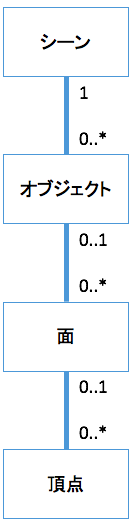
\includegraphics[scale=0.5]{images/er}
    \caption{データモデル間の依存関係}
    \label{データ構造}
  \end{center}
\end{figure}
図\ref{データ構造}のようにシーンのデータモデルはオブジェクトを, オブジェクトは面を, 面は頂点をそれぞれ子にもつ. また, 子のみが親の参照先をもつ.
各データモデルのパラメータを図\ref{パラメータ}に示す.
\begin{figure}[]
  \begin{center}
    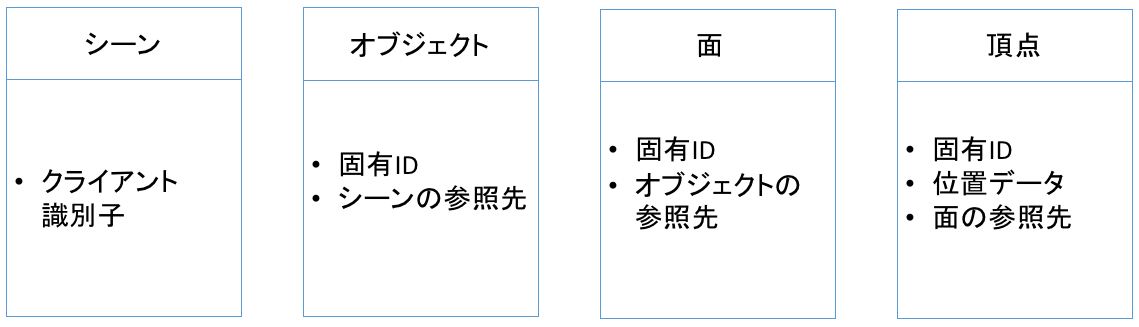
\includegraphics[scale=0.3]{images/prop}
    \caption{データモデルがもつパラメータ}
    \label{パラメータ}
  \end{center}
\end{figure}
シーンはクライアント識別子というパラメータを持ちサーバシャドウの役割を担う.
またシーンのクライアント識別子に0を与えサーバデータとする.
これらのデータ構造によって, 子を削除した場合に親との依存関係も削除できる.
親を新しく参照する場合, 子のデータを複製しながら新しく参照する親を参照先に追加する.
子のデータを複製していくことによって, 関係を削除した際も複製元のデータは残る.
%%%%%%%%%%%%%%%%%%%%%%%%%%%%%%%%%%
%    固有IDの付与
%%%%%%%%%%%%%%%%%%%%%%%%%%%%%%%%%%
\section{固有IDの付与} \label{固有id}
各データには, 複数クライアント間でIDの衝突が起こるのを防ぐため, そのデータを作成したクライアント識別子を組み込んだ固有IDを与える.
本システムでは図\ref{uuid}のように, クライアント識別子およびデータモデル識別子, インクリメント番号, ランダム文字列の順につなげた固有IDを与える. クライアント識別子は1から順に振られたユーザIDを用いてクライアントが付与する. また, データモデル識別子は, オブジェクトが0, 面は1, 頂点は2となるように与える.
インクリメント番号は, サーバでもクライアントでも作ったデータの数を記憶しておき, 作るごとにインクリメントする番号である. ランダム文字列は3桁の数字またはアルファベットからなる文字列であり, 固有IDの競合の発生を抑制する.
\begin{figure}[]
  \begin{center}
    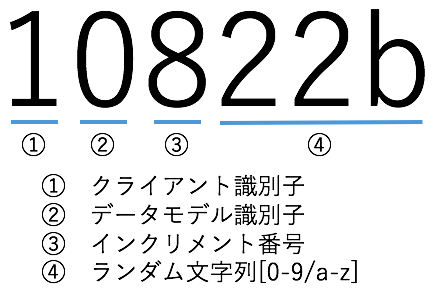
\includegraphics[scale=0.5]{images/uuid}
    \caption{本システムの固有ID}
    \label{uuid}
  \end{center}
\end{figure}

%%%%%%%%%%%%%%%%%%%%%%%%%%%%%%%%%%
%    同期の手順
%%%%%%%%%%%%%%%%%%%%%%%%%%%%%%%%%%
\section{同期の手順}
同期はDifferential Synchronizationに基づいて行う.
同期の手順を図\ref{differential}を用いて説明する. なお,図\ref{differential}中の各番号は処理の順番を表している. まず(1)クライアントデータとそのシャドウコピーの差分を計算し, (2)サーバに送信する. 次に, クライアントでは(3)シャドウコピーを更新し, サーバで(4)適用処理を行う. サーバ側でも同様の手順で処理することで同期が可能となる. サーバデータは複数のクライアントから利用され, クライアントデータと2つのシャドウコピーは接続しているクライアントごとに用意される.
\begin{figure}[]
  \begin{center}
    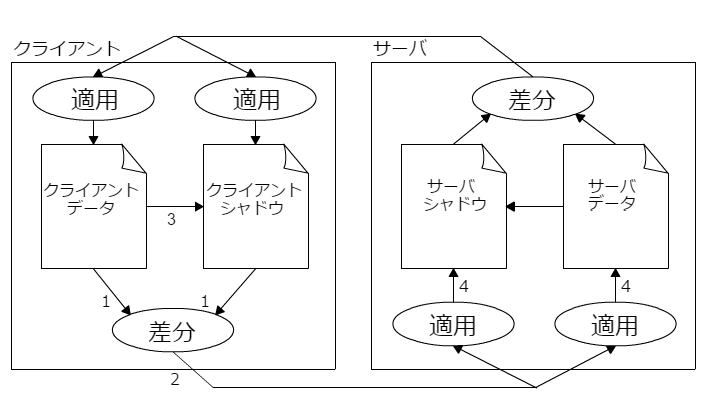
\includegraphics[scale=0.7]{images/DS}
    \caption{Differential Synchronization}
    \label{differential}
  \end{center}
\end{figure}
\par
% 本来, 変数v1を変数v2にコピーするならばv2 = v1のように代入することで実装する. しかし, 本システムではデータをデータベースに登録して管理しており, 単純な代入で処理できない.
% また, 元のデータを削除し新しくシャドウコピーを作成する方法は, 頻繁にシャドウコピーを作成するDifferential Synchronizationでは,
% データベースのDELETE命令とCREATE命令を頻発させることになり, 処理においてボトルネックとなってしまう.
サーバデータを全てサーバシャドウとしてコピーするにはデータ量の負担が大きいため, サーバでのコピーは, サーバデータとサーバシャドウの差分を取り, サーバシャドウに適用することによって解決する.
\par
1つのサーバに対し2つのクライアントの同期の具体的な例を図\ref{sycle1}から図\ref{sycle3}を用いて説明する. まずクライアントAの同期の手順を図\ref{sycle1}に示す.
クライアントAが頂点を作成する編集を行うと, クライアントAのクライアントデータに``122xyz''が作成されたとする(図\ref{sycle1}(a)). クライアントAでは, クライアントデータとクライアントシャドウの差分を計算し, [+ ``122xyz'']となる. 次に, 計算した差分をサーバに送信し, [+ ``122xyz'']をクライアントAのサーバシャドウと, サーバデータに適用する(図\ref{sycle1}(b)). この時にクライアントAでは, クライアントデータをクライアントシャドウにコピーする(図\ref{sycle1}(c)). サーバでは受信したデータの適用後, サーバデータとサーバシャドウとの差分を計算し, 差分なし[ ]となる(図\ref{sycle1}(d)). この時にサーバではサーバデータをクライアントAのサーバシャドウにコピーする(図\ref{sycle1}(e)).
クライアントBの同期の手順を図\ref{sycle2}に示す.
クライアントBがすでにある頂点を削除する編集を行うと, クライアントBのクライアントデータにある``121abc''が削除されたとする(図\ref{sycle2}(a)).
クライアントBはクライアントデータとクライアントシャドウの差分を計算し, [-- ``121abc'']となる. 次に, 計算した差分をサーバに送信し, [-- ``121abc'']をクライアントBのサーバシャドウと, サーバデータに適用する(図\ref{sycle2}(b)). その時クライアントBではシャドウコピーを作成する(図\ref{sycle2}(c)). サーバでは差分を計算し, [+ ``122xyz'']となる. [+ ``122xyz'']をクライアントBのクライアントデータとクライアントシャドウに適用する(図\ref{sycle2}(d)). この時にサーバではシャドウコピーを作成する(図\ref{sycle2}(e)).
またクライアントBの編集をクライアントAが検知して, 各クライアント間でデータが一致するまでの手順を図\ref{sycle3}に示す.
まず, クライアントAが差分を計算し差分なし[ ]となる(図\ref{sycle3}(a)).
差分なし[ ]なので, サーバデータとサーバシャドウに適用するものはない(図\ref{sycle3}(b)). その時にクライアントAではシャドウコピーを作成する(図\ref{sycle2}(c)).
次に, サーバデータとサーバシャドウの差分を計算し, [-- ``121abc'']となる\ref{sycle3}(d)). 計算した差分をクライアントに送信し, [-- ``121abc'']をクライアントAのクライアントデータとクライアントシャドウに適用する.
この手順により各クライアントのクライアントデータ, クライアントシャドウ, サーバのサーバデータとサーバシャドウのデータが一致し, 同期が可能となる.

\begin{figure}[]
  \begin{center}
    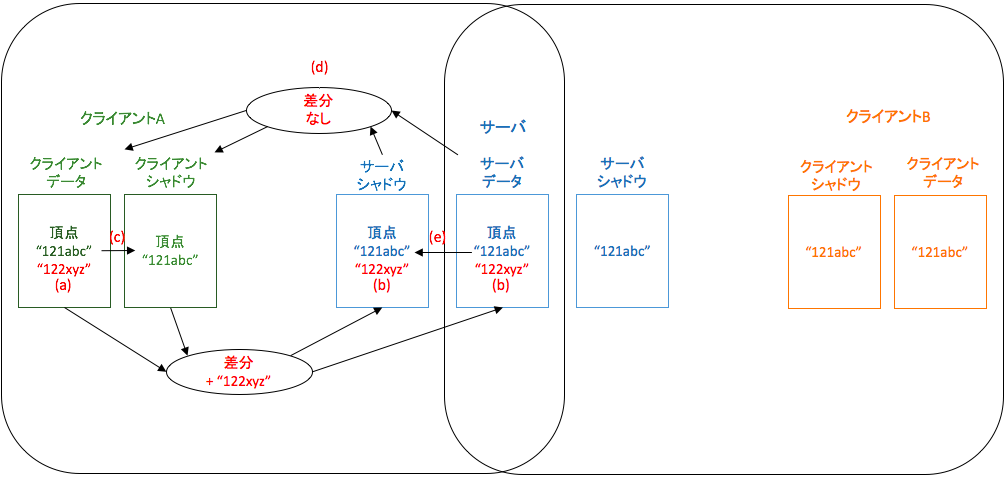
\includegraphics[scale=0.45]{images/sycle1}
    \caption{クライアントAの同期の手順}
    \label{sycle1}
  \end{center}
\end{figure}
\begin{figure}[]
  \begin{center}
    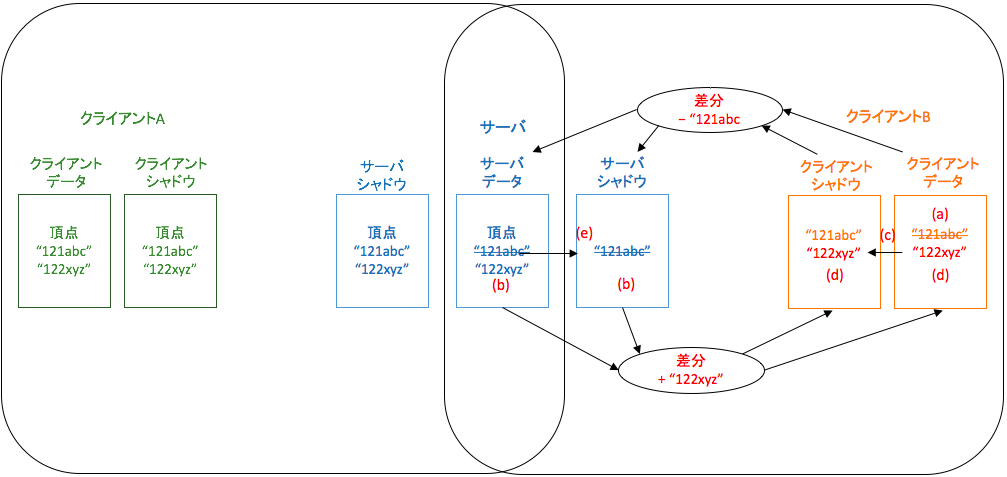
\includegraphics[scale=0.45]{images/sycle2}
    \caption{クライアントBの同期の手順}
    \label{sycle2}
  \end{center}
\end{figure}
\begin{figure}[]
  \begin{center}
    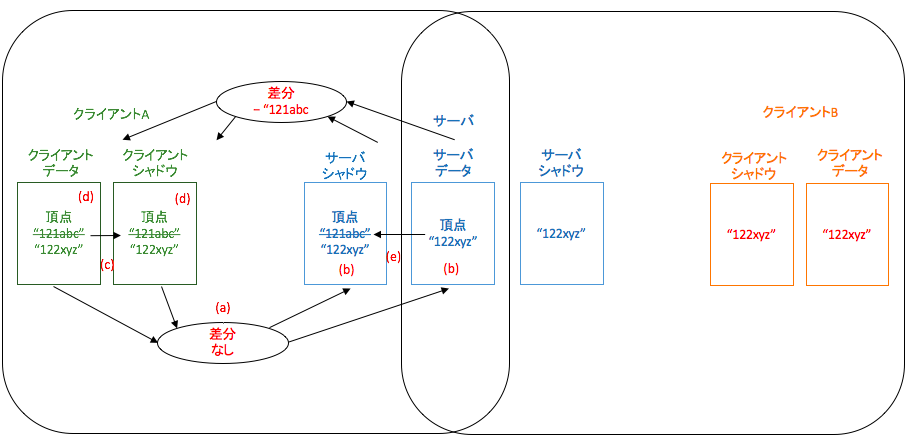
\includegraphics[scale=0.5]{images/sycle3}
    \caption{2回目のクライアントAの同期の手順}
    \label{sycle3}
  \end{center}
\end{figure}
%%%%%%%%%%%%%%%%%%%%%%%%%%%%%%%%%%
%    基本命令
%%%%%%%%%%%%%%%%%%%%%%%%%%%%%%%%%%
\section{基本命令} \label{ope}
オブジェクト, 面, 頂点の各データモデルに対して, 作成, 親への参照の追加, 削除の3つの基本命令を定義する.
基本命令はシステムに対する最低限の命令であり, これらの命令を組み合わせることで, 3Dモデリングで使われる面の分割や押し出しなど, より高度な命令を実現できる.
基本命令を適用する際のデータの変化を図\ref{命令0}から図\ref{命令5}を用いて説明する.
まず最初のデータとして図\ref{命令0}のように, 面が1つ, 頂点が2つあり, 一方の頂点が面を参照しているとする.
\begin{figure}[]
  \begin{center}
    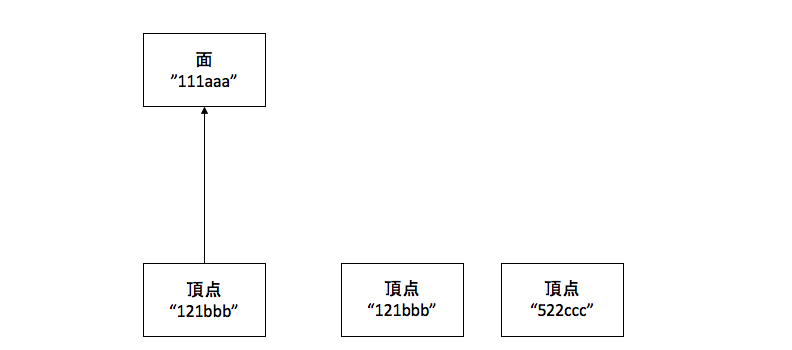
\includegraphics[scale=0.45]{images/ope0}
    \caption{最初のデータ}
    \label{命令0}
  \end{center}
\end{figure}
図\ref{命令0}のデータに対して, 頂点の作成命令を適用した場合のデータの変化を図\ref{命令1}に示す. 図\ref{命令1}は頂点``123ddd''を作成した.
\begin{figure}[]
  \begin{center}
    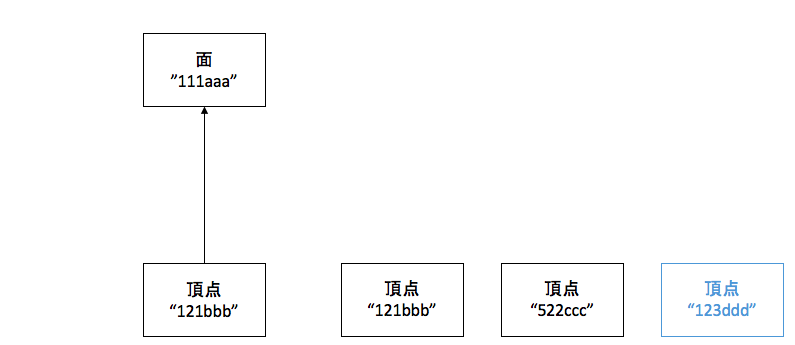
\includegraphics[scale=0.45]{images/ope1}
    \caption{作成命令適用後}
    \label{命令1}
  \end{center}
\end{figure}
図\ref{命令1}の頂点``522ccc''に対して, 面``111aaa''を親とする参照の追加命令を適用した場合のデータの変化を図\ref{命令2}に示す. 図\ref{命令2}は子である頂点``522ccc''を複製しながら面への参照をする.
\begin{figure}[]
  \begin{center}
    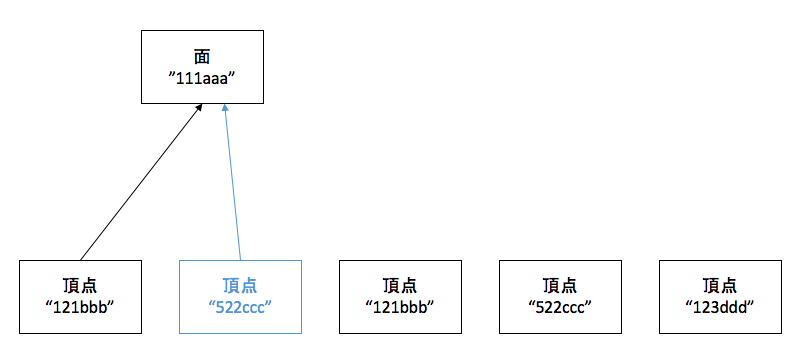
\includegraphics[scale=0.45]{images/ope2}
    \caption{親への参照追加命令適用後}
    \label{命令2}
  \end{center}
\end{figure}
図\ref{命令2}の頂点``123ddd''に対して, 削除命令を適用した場合のデータの変化を図\ref{命令3}に示す. 図\ref{命令3}は, 頂点``123ddd''が削除される.
\begin{figure}[]
  \begin{center}
    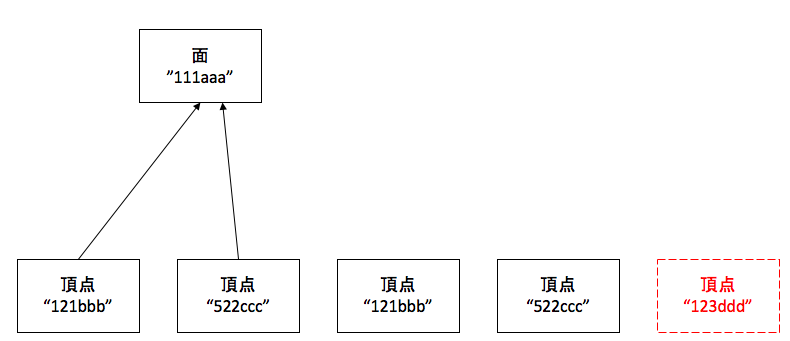
\includegraphics[scale=0.45]{images/ope3}
    \caption{削除命令適用後}
    \label{命令3}
  \end{center}
\end{figure}
図\ref{命令3}の頂点``522ccc''に対して, 削除命令を適用した場合のデータの変化を図\ref{命令4}に示す. 図\ref{命令4}は, 頂点``522ccc''であるデータが複数あるが, 全ての 頂点``522ccc''に関するデータを削除する. この際に, 子が親の参照先を持っているので, 参照関係も同時に消える.
\begin{figure}[]
  \begin{center}
    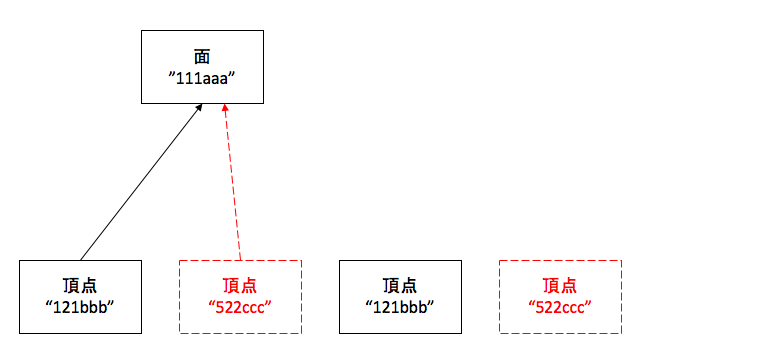
\includegraphics[scale=0.45]{images/ope4}
    \caption{参照関係を含んだデータの削除命令適用後}
    \label{命令4}
  \end{center}
\end{figure}
図\ref{命令4}のデータである面``111aaa''に対して, 削除命令を適用した場合のデータの変化を図\ref{命令5}に示す. 図\ref{命令5}は, 面``111aaa''を削除し, それを参照している子のデータも一緒に削除する. この際, 参照がないデータは削除しない.
\begin{figure}[]
  \begin{center}
    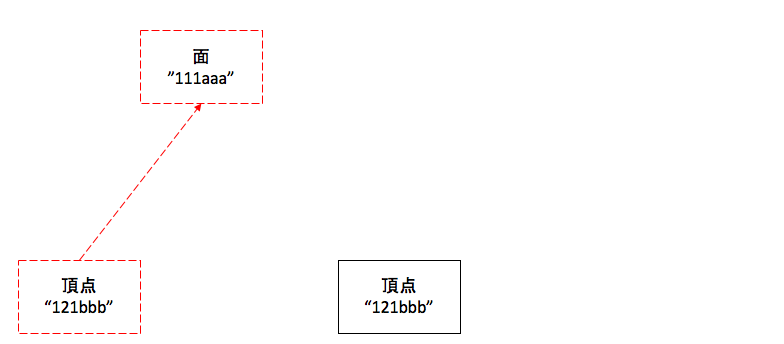
\includegraphics[scale=0.45]{images/ope5}
    \caption{親のデータの削除命令適用後}
    \label{命令5}
  \end{center}
\end{figure}
削除命令や親への参照の追加をする命令を適用する際, 命令の対象がない場合は適用を無効とする.
